\documentclass[]{book}
\usepackage{lmodern}
\usepackage{amssymb,amsmath}
\usepackage{ifxetex,ifluatex}
\usepackage{fixltx2e} % provides \textsubscript
\ifnum 0\ifxetex 1\fi\ifluatex 1\fi=0 % if pdftex
  \usepackage[T1]{fontenc}
  \usepackage[utf8]{inputenc}
\else % if luatex or xelatex
  \ifxetex
    \usepackage{mathspec}
  \else
    \usepackage{fontspec}
  \fi
  \defaultfontfeatures{Ligatures=TeX,Scale=MatchLowercase}
\fi
% use upquote if available, for straight quotes in verbatim environments
\IfFileExists{upquote.sty}{\usepackage{upquote}}{}
% use microtype if available
\IfFileExists{microtype.sty}{%
\usepackage{microtype}
\UseMicrotypeSet[protrusion]{basicmath} % disable protrusion for tt fonts
}{}
\usepackage[margin=1in]{geometry}
\usepackage{hyperref}
\hypersetup{unicode=true,
            pdftitle={YaRrr! The Pirate's Guide to R},
            pdfauthor={Nathaniel D. Phillips},
            pdfborder={0 0 0},
            breaklinks=true}
\urlstyle{same}  % don't use monospace font for urls
\usepackage{natbib}
\bibliographystyle{apalike}
\usepackage{longtable,booktabs}
\usepackage{graphicx,grffile}
\makeatletter
\def\maxwidth{\ifdim\Gin@nat@width>\linewidth\linewidth\else\Gin@nat@width\fi}
\def\maxheight{\ifdim\Gin@nat@height>\textheight\textheight\else\Gin@nat@height\fi}
\makeatother
% Scale images if necessary, so that they will not overflow the page
% margins by default, and it is still possible to overwrite the defaults
% using explicit options in \includegraphics[width, height, ...]{}
\setkeys{Gin}{width=\maxwidth,height=\maxheight,keepaspectratio}
\IfFileExists{parskip.sty}{%
\usepackage{parskip}
}{% else
\setlength{\parindent}{0pt}
\setlength{\parskip}{6pt plus 2pt minus 1pt}
}
\setlength{\emergencystretch}{3em}  % prevent overfull lines
\providecommand{\tightlist}{%
  \setlength{\itemsep}{0pt}\setlength{\parskip}{0pt}}
\setcounter{secnumdepth}{5}
% Redefines (sub)paragraphs to behave more like sections
\ifx\paragraph\undefined\else
\let\oldparagraph\paragraph
\renewcommand{\paragraph}[1]{\oldparagraph{#1}\mbox{}}
\fi
\ifx\subparagraph\undefined\else
\let\oldsubparagraph\subparagraph
\renewcommand{\subparagraph}[1]{\oldsubparagraph{#1}\mbox{}}
\fi

%%% Use protect on footnotes to avoid problems with footnotes in titles
\let\rmarkdownfootnote\footnote%
\def\footnote{\protect\rmarkdownfootnote}

%%% Change title format to be more compact
\usepackage{titling}

% Create subtitle command for use in maketitle
\newcommand{\subtitle}[1]{
  \posttitle{
    \begin{center}\large#1\end{center}
    }
}

\setlength{\droptitle}{-2em}
  \title{YaRrr! The Pirate's Guide to R}
  \pretitle{\vspace{\droptitle}\centering\huge}
  \posttitle{\par}
  \author{Nathaniel D. Phillips}
  \preauthor{\centering\large\emph}
  \postauthor{\par}
  \predate{\centering\large\emph}
  \postdate{\par}
  \date{2017-03-17}

\usepackage{booktabs}
\usepackage{amsthm}
\makeatletter
\def\thm@space@setup{%
  \thm@preskip=8pt plus 2pt minus 4pt
  \thm@postskip=\thm@preskip
}
\makeatother

\usepackage{amsthm}
\newtheorem{theorem}{Theorem}[chapter]
\newtheorem{lemma}{Lemma}[chapter]
\theoremstyle{definition}
\newtheorem{definition}{Definition}[chapter]
\newtheorem{corollary}{Corollary}[chapter]
\newtheorem{proposition}{Proposition}[chapter]
\theoremstyle{definition}
\newtheorem{example}{Example}[chapter]
\theoremstyle{remark}
\newtheorem*{remark}{Remark}
\begin{document}
\maketitle

{
\setcounter{tocdepth}{1}
\tableofcontents
}
\chapter{Preface}\label{intro}

\chapter{Getting Started}\label{started}

\chapter{Jump In!}\label{jumpin}

\chapter{The Basics}\label{basics}

\chapter{Scalers and vectors}\label{scalersvectors}

\chapter{Vector functions}\label{vectorfunctions}

\chapter{Indexing Vectors with {[} {]}}\label{vectorindexing}

\chapter{Matrices and Dataframes}\label{matricesdataframes}

\chapter{Importing, saving and managing data}\label{importingdata}

\chapter{Advanced dataframe manipulation}\label{advanceddataframe}

\chapter{Plotting (I)}\label{plotting1}

\chapter{Plotting (II)}\label{plotting2}

\chapter{Hypothesis Tests}\label{htests}

\chapter{ANOVA}\label{anova}

\chapter{Regression}\label{regression}

\begin{verbatim}
## 
## Attaching package: 'dplyr'
\end{verbatim}

\begin{verbatim}
## The following objects are masked from 'package:stats':
## 
##     filter, lag
\end{verbatim}

\begin{verbatim}
## The following objects are masked from 'package:base':
## 
##     intersect, setdiff, setequal, union
\end{verbatim}

\begin{verbatim}
## Loading required package: jpeg
\end{verbatim}

\begin{verbatim}
## Loading required package: BayesFactor
\end{verbatim}

\begin{verbatim}
## Loading required package: coda
\end{verbatim}

\begin{verbatim}
## Loading required package: Matrix
\end{verbatim}

\begin{verbatim}
## ************
## Welcome to BayesFactor 0.9.12-2. If you have questions, please contact Richard Morey (richarddmorey@gmail.com).
## 
## Type BFManual() to open the manual.
## ************
\end{verbatim}

\begin{verbatim}
## yarrr v0.1.5. Citation info at citation('yarrr'). Package guide at yarrr.guide()
\end{verbatim}

\begin{verbatim}
## Email me at Nathaniel.D.Phillips.is@gmail.com
\end{verbatim}

\begin{figure}

{\centering 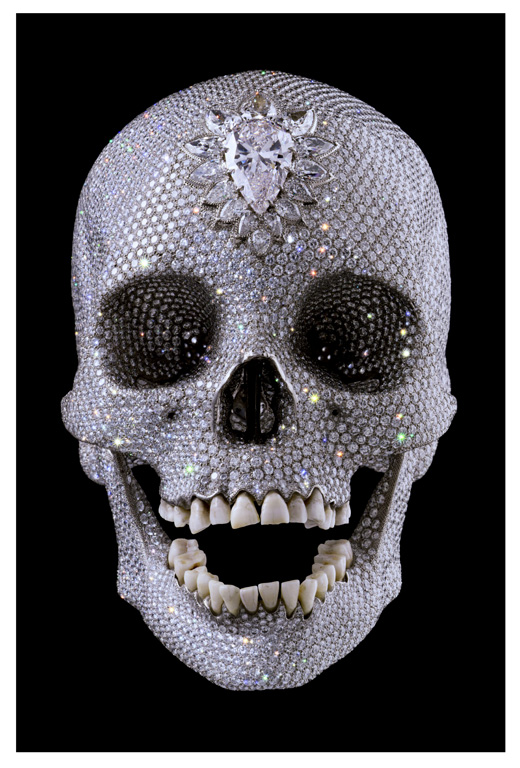
\includegraphics[width=0.2\linewidth]{images/diamondskull} 

}

\caption{Insert funny caption here.}\label{fig:unnamed-chunk-2}
\end{figure}

Pirates like diamonds. Who doesn't?! But as much as pirates love
diamonds, they hate getting ripped off. For this reason, a pirate needs
to know how to accurately assess the value of a diamond. For example,
how much should a pirate pay for a diamond with a weight of 2.0 grams, a
clarity value of 1.0, and a color gradient of 4 out of 10? To answer
this, we'd like to know how the attributes of diamonds (e.g.; weight,
clarity, color) relate to its value. We can get these values using
linear regression.

\section{The Linear Model}\label{the-linear-model}

The linear model is easily the most famous and widely used model in all
of statistics. Why? Because it can apply to so many interesting research
questions where you are trying to predict a continuous variable of
interest (the \emph{response} or \emph{dependent variable}) on the basis
of one or more other variables (the \emph{predictor} or
\emph{independent variables}).

The linear model takes the following form, where the x values represent
the predictors, while the beta values represent weights.

\(y=\beta_{0}+\beta_{1}x_{1}+\beta_{2}x_{2}+...\beta_{n}x_{n}\)

For example, we could use a regression model to understand how the value
of a diamond relates to two independent variables: its weight and
clarity. In the model, we could define the value of a diamond as
\(\beta_{weight} \times weight + \beta{clarity} \times clarity\). Where
\(\beta_{weight}\) indicates how much a diamond's value changes as a
function of its weight, and \(\beta_{clarity}\) defines how much a
diamond's value change as a function of its clarity.

\section{\texorpdfstring{Linear regression with
\texttt{lm()}}{Linear regression with lm()}}\label{linear-regression-with-lm}

To estimate the beta weights of a linear model in R, we use the
\texttt{lm()} function. The function has three key arguments:
\texttt{formula}, and \texttt{data}

\chapter{Solutions}\label{solutions}

\chapter{Placeholder}\label{placeholder}

\bibliography{packages.bib,book.bib}


\end{document}
